% ============================================================================
% MÓDULO 2 — ABERTURA E CAPÍTULO 5
% CHF662 — ANÁLISE AMBIENTAL (DCHF/UEFS)
% ============================================================================

\aberturaModulo{MÓDULO 2}{AVALIAÇÃO DE IMPACTO AMBIENTAL E ANÁLISE INTEGRADA}{Semanas 5 e 6 $\bullet$ Base do Estudo Orientado EO4, Prova Teórica e Trabalho Final}{%
  O Módulo 2 estabelece a passagem entre os fundamentos epistemológicos e conceituais estudados no Módulo 1 e a prática técnica da Análise Ambiental aplicada ao território. Nas próximas duas semanas letivas, você aprenderá a antecipar consequências de intervenções humanas antes que os danos se tornem irreversíveis e a integrar processos físico-bióticos e socioespaciais sob uma perspectiva sistêmica e multiescalar.

  \vspace{4pt}
  \begin{itemize}[leftmargin=1.5em, itemsep=3pt]
    \item \textbf{Capítulo 5, Avaliação de Impacto Ambiental (AIA) e Planejamento Ambiental (Semana 5 $\bullet$ Base do EO4):} natureza preventiva da AIA, encadeamento completo de etapas (triagem, escopo, diagnóstico, áreas de influência, métodos de identificação e previsão, prognóstico, hierarquia de mitigação, compensação, Plano Básico Ambiental e monitoramento), com demonstração numérica de matrizes ponderadas.
    \item \textbf{Capítulo 6, Fundamentos da Análise Ambiental Integrada, Escalas e Ordenamento Territorial (Semana 6):} interações funcionais entre os meios físico, biótico e antrópico, acoplamento entre escalas espaciais e temporais, falácia de escala, sistemas ambientais abertos, balanços de massa, limiares (\textit{thresholds}), retroalimentação e Zoneamento Ecológico-Econômico (ZEE).
    \item \textbf{Simulado e Revisão Integrada do Módulo 2:} 8 questões objetivas autorais no estilo ENADE e concursos ambientais, 2 questões dissertativas no formato da Avaliação Teórica da disciplina, gabarito comentado, espelho dissertativo e tabela de diagnóstico de revisão.
  \end{itemize}
}

\chapter{Avaliação de Impacto Ambiental (AIA) e Planejamento Ambiental}
\label{cap:aia}

\noindent\tagEmenta\ \tagEO{4}\ \tagPratica
\par\vspace{6pt}

% ============================================================================
% ETAPA 1 — OBJETIVOS
% ============================================================================
\begin{capObjetivos}
  Ao concluir este capítulo, você será capaz de:
  \begin{itemize}[leftmargin=1.5em, itemsep=2.5pt]
    \item Explicar o conceito, a finalidade preventiva e o papel da Avaliação de Impacto Ambiental (AIA) no planejamento e no licenciamento ambiental, diferenciando AIA de EIA/RIMA.
    \item Descrever em sequência lógica as etapas do processo de AIA, abrangendo triagem (\textit{screening}), definição de escopo (\textit{scoping} e Termo de Referência), diagnóstico ambiental, delimitação de áreas de influência (ADA, AID e AII), identificação e previsão de impactos, prognóstico, mitigação, compensação, Plano Básico Ambiental (PBA) e monitoramento pós-implantação.
    \item Aplicar e interpretar os principais métodos de identificação e valoração de impactos, incluindo listagens de controle (\textit{checklists}), Matriz de Leopold e matrizes ponderadas, redes de interação e sobreposição de cartas em SIG.
    \item Empregar a Hierarquia de Mitigação (\textbf{Evitar $\to$ Minimizar $\to$ Recuperar $\to$ Compensar}) para ordenar decisões técnicas e distinguir medidas mitigadoras de compensatórias.
    \item Avaliar criticamente a efetividade de programas de monitoramento no PBA, utilizando indicadores quantitativos de linha de base e metas ambientais auditáveis.
  \end{itemize}
\end{capObjetivos}

% ============================================================================
% ETAPA 2 — REVISÃO
% ============================================================================
\begin{capRevisao}
  Antes de avançar para os instrumentos da AIA, retome quatro noções consolidadas no Módulo 1 (especialmente no Capítulo 4):
  \begin{enumerate}[leftmargin=1.6em, itemsep=2.5pt]
    \item \textbf{Aspecto ambiental versus impacto ambiental:} o \emph{aspecto} corresponde à causa ligada à atividade humana (por exemplo, supressão de vegetação ou lançamento de efluente), enquanto o \emph{impacto} designa a alteração resultante na qualidade ambiental (como perda de solo por erosão ou eutrofização), podendo ser adverso ou benéfico.
    \item \textbf{Degradação ambiental:} alteração adversa dos processos, funções ou componentes ambientais que reduz a capacidade do sistema de sustentar a biodiversidade e os serviços ecossistêmicos. Todo processo de degradação decorre de impactos adversos, embora nem todo impacto produza degradação irreversível.
    \item \textbf{Vulnerabilidade, fragilidade e risco:} a fragilidade refere-se à suscetibilidade intrínseca e emergente do meio físico-biótico; a vulnerabilidade expressa o grau de exposição e suscetibilidade social ou ecológica diante de um perigo; o risco combina perigo e vulnerabilidade.
    \item \textbf{Política Nacional do Meio Ambiente (PNMA, Lei nº 6.938/1981):} instituiu a AIA como um de seus instrumentos centrais, posteriormente regulamentada pelas Resoluções CONAMA nº 001/1986 e nº 237/1997.
  \end{enumerate}
\end{capRevisao}

% ============================================================================
% ETAPA 3 — EXPLICAÇÃO TEÓRICA E EXEMPLOS INTERCALADOS
% ============================================================================
\etapa{3}{Fundamentação Teórica: Processo de AIA, Métodos e Mitigação}

\begin{boxSimbolo}[Vocabulário Técnico e Siglas Essenciais da AIA]
  Na análise de empreendimentos, a \textbf{Avaliação de Impacto Ambiental (AIA)} designa o processo sistemático e preventivo que examina as consequências futuras de uma proposta antes da decisão administrativa. Quando há potencial de significativa degradação, o processo concretiza-se no \textbf{Estudo de Impacto Ambiental (EIA)}, documento técnico completo, acompanhado pelo \textbf{Relatório de Impacto Ambiental (RIMA)}, sua síntese acessível à sociedade. O escopo e o detalhamento exigidos constam no \textbf{Termo de Referência (TR)}, emitido pelo órgão licenciador. Espacialmente, os levantamentos distinguem a \textbf{Área Diretamente Afetada (ADA)}, a \textbf{Área de Influência Direta (AID)} e a \textbf{Área de Influência Indireta (AII)} para os meios físico, biótico e socioeconômico. Na etapa executiva, o \textbf{Plano Básico Ambiental (PBA)} organiza os programas de controle e monitoramento. Nas matrizes ponderadas adaptadas de Leopold, cada interação entre o fator $i$ e a ação $j$ recebe sinal ($s_{ij}$), magnitude ($M_{ij}$, de $1$ a $10$), importância ($I_{ij}$, de $1$ a $10$) e pontuação ponderada $P_{ij} = s_{ij} \cdot M_{ij} \cdot I_{ij}$, enquanto a parcela inevitável após todas as intervenções de controle recebe o nome de \textbf{impacto residual}.
\end{boxSimbolo}

\section{Conceito, Natureza Preventiva e Papel da AIA no Planejamento}

A \textbf{Avaliação de Impacto Ambiental (AIA)} opera como um instrumento de política e planejamento ambiental de caráter preventivo. Como sintetiza Sánchez (2013, cap. 7), avaliar impactos ambientais significa identificar, prever, interpretar e comunicar, \emph{antes} que uma obra, atividade ou política seja implantada, as alterações que ela poderá provocar nos meios físico, biótico e socioeconômico, propondo medidas capazes de evitar ou reduzir danos e ampliar benefícios.

No Brasil, a AIA integra os instrumentos da Política Nacional do Meio Ambiente (Lei nº 6.938/1981) e articula-se diretamente ao licenciamento ambiental (Brasil/MMA, 2016; Vital et al., 2020). O Estudo de Impacto Ambiental e seu respectivo Relatório (EIA/RIMA) representam a modalidade mais completa desse processo, exigida para empreendimentos potencialmente causadores de significativa degradação ambiental conforme a Resolução CONAMA nº 001/1986. Além do EIA/RIMA, o processo de AIA abrange estudos simplificados (como o Relatório Ambiental Simplificado, o Plano de Controle Ambiental e o Estudo Ambiental Preliminar), o exame técnico pelo órgão licenciador, as audiências públicas e o acompanhamento posterior à concessão da licença.

\subsection{A AIA como Instrumento do Planejamento Ambiental}

Quando reduzida a um rito cartorial executado depois que todas as decisões de engenharia já estão fechadas, a AIA perde sua função preventiva e converte-se em justificativa documental tardia. Para cumprir seu papel no \textbf{planejamento ambiental}, o estudo precisa atuar desde a concepção do projeto, orientando três decisões estruturantes. No plano espacial, subsidia a comparação de \textbf{alternativas locacionais}, definindo onde instalar a infraestrutura para resguardar nascentes, Áreas de Preservação Permanente (APPs), solos suscetíveis à erosão e territórios de elevado valor sociocultural. De forma complementar, orienta a seleção de \textbf{alternativas tecnológicas}, contrastando métodos construtivos e processos produtivos para escolher aqueles que geram menor volume de rejeitos, menor supressão vegetal e menor demanda hídrica. Simultaneamente, exige a avaliação da \textbf{alternativa zero}, referente à manutenção do território sem a obra, verificando se o interesse público e o balanço socioambiental justificam a intervenção proposta.

A distinção entre o processo amplo de avaliação e suas peças documentais previne equívocos frequentes no licenciamento, conforme destacado a seguir.

\begin{boxErro}[Erro 1: Confundir AIA com EIA/RIMA ou Tratar o Licenciamento como Burocracia]
  \textbf{Equívoco frequente:} Afirmar que ``todo licenciamento exige EIA/RIMA'' ou empregar AIA e EIA como sinônimos exatos.\par
  \textbf{Correção técnica:} A AIA corresponde ao \emph{processo amplo} de avaliação prévia de impactos (triagem, escopo, estudos, decisão e acompanhamento), enquanto o EIA/RIMA constitui uma de suas \emph{modalidades documentais}, exigida quando há potencial de significativa degradação ambiental. Empreendimentos de menor porte ou potencial poluidor passam pela etapa de triagem e apresentam estudos simplificados, como o Relatório Ambiental Simplificado (RAS) ou o Plano de Controle Ambiental (PCA).
\end{boxErro}

\section{Etapas do Processo de Avaliação de Impacto Ambiental}

A literatura internacional e os manuais brasileiros de referência (Sánchez, 2013; Brasil/MMA, 2016) organizam a AIA em um encadeamento lógico e iterativo de etapas no qual cada fase condiciona a consistência da etapa seguinte, como se observa no Painel (a) da Figura~\ref{fig:aia_mitigacao}.

\begin{figure}[htbp]
  \centering
  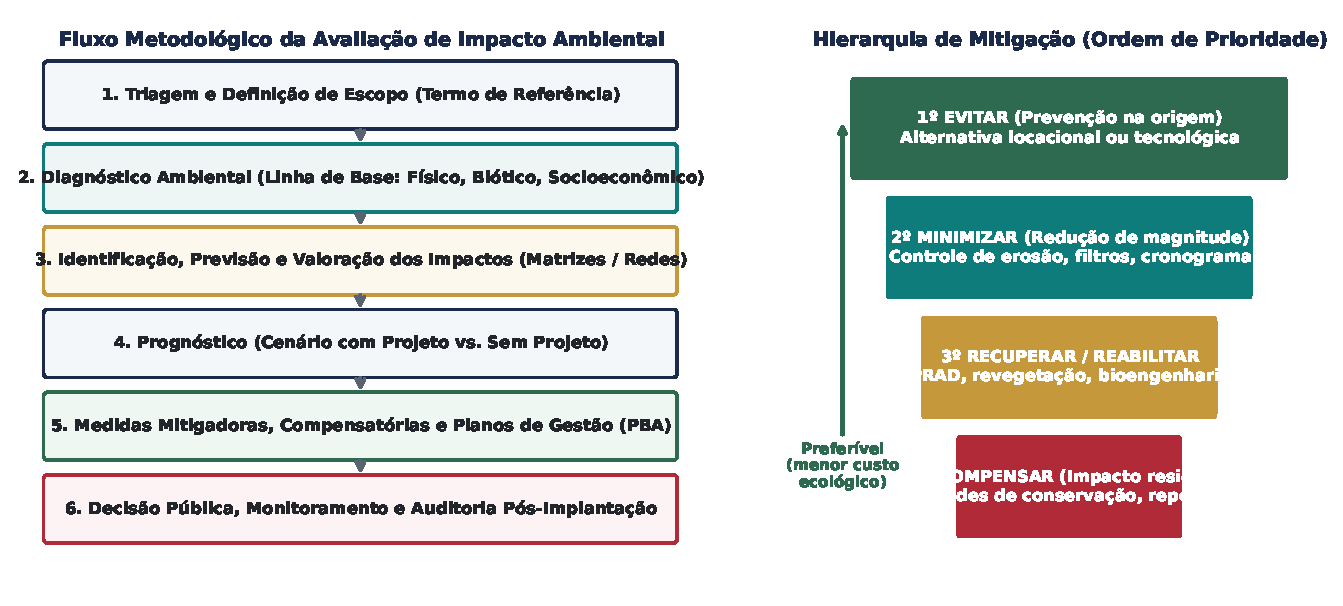
\includegraphics[width=0.95\textwidth]{figures/fig03_etapas_aia_mitigacao.pdf}
  \caption{Fluxo metodológico da Avaliação de Impacto Ambiental (a) e ordem de prioridade técnica da Hierarquia de Mitigação (b). Fonte: elaboração didática CHF662 com base em Sánchez (2013) e Brasil/MMA (2016).}
  \label{fig:aia_mitigacao}
\end{figure}

\subsection{Triagem e Definição de Escopo (Termo de Referência)}

A \textbf{triagem (\textit{screening})} abre o processo ao responder se o projeto requer EIA/RIMA completo, estudo ambiental simplificado ou dispensa de AIA. Essa decisão combina a tipologia da atividade (rodovias, parques eólicos, mineração ou barragens), o porte do empreendimento (área ocupada, potência instalada ou vazão captada) e a \textbf{sensibilidade ambiental do sítio}, avaliando a proximidade de Unidades de Conservação, terras indígenas, comunidades tradicionais, nascentes ou remanescentes de Caatinga conservada.

Confirmada a exigência de estudo ambiental, a \textbf{definição de escopo (\textit{scoping})} delimita os temas e processos que exigem investigação aprofundada, evitando relatórios extensos repletos de dados secundários desconexos e estudos omissos quanto aos riscos principais. O produto formal dessa etapa é o \textbf{Termo de Referência (TR)}, emitido pelo órgão ambiental competente (como o INEMA na Bahia ou o IBAMA na esfera federal) ou estruturado como proposta técnica pelo consultor para validação prévia.

Na prática profissional, uma proposta consistente de Termo de Referência encadeia cinco blocos integrados. O bloco inicial fixa a abrangência do estudo (EIA, RIMA e, quando houver risco químico ou tecnológico, Estudo de Análise de Risco) e exige levantamentos primários em campo articulados a bases oficiais recentes (IBGE, INEMA, ANA e universidades), com protocolos explícitos de amostragem. O bloco seguinte caracteriza o empreendimento por meio de cadastro técnico, histórico da área, mapa de localização em escala de detalhe (como $1{:}10.000$) inserido na bacia hidrográfica, mapa de restrições legais e descrição operacional de insumos, resíduos sólidos (ABNT NBR 10004 a 10007), efluentes, ruído e tráfego.

Em seguida, o TR especifica os parâmetros mínimos do diagnóstico na AID e na AII em escalas cartográficas compatíveis, usualmente $1{:}25.000$ para a AID e $1{:}50.000$ para a AII. Esse diagnóstico cobre geologia, geomorfologia, hidrografia e qualidade do ar no meio físico; inventários florísticos e faunísticos com curvas de suficiência amostral no meio biótico; e dinâmica demográfica, uso do solo, anuência do IPHAN para patrimônio arqueológico e levantamento específico de povos indígenas e comunidades quilombolas segundo registros da Fundação Cultural Palmares e do INCRA no meio socioeconômico. No bloco final, o documento define o método de valoração de impactos, os programas ambientais do PBA com cronograma e orçamento, as cartas temáticas sobre base planialtimétrica comum, as diretrizes de redação acessível do RIMA, as Anotações de Responsabilidade Técnica (ARTs) da equipe e os procedimentos de consulta pública.

\subsection{Diagnóstico Ambiental (Linha de Base) e Áreas de Influência}

O diagnóstico constrói a \textbf{linha de base (\textit{baseline})}, retratando de modo qualiquantitativo as condições do ambiente antes da intervenção. No \textbf{meio físico}, levantam-se clima, geologia, geomorfologia, solos, recursos hídricos superficiais e subterrâneos, qualidade do ar e ruído de fundo para aferir a suscetibilidade do substrato à erosão e às alterações hidrológicas. No \textbf{meio biótico}, inventariam-se fitofisionomias, flora (com atenção a espécies endêmicas e ameaçadas), fauna terrestre e aquática e corredores ecológicos. No \textbf{meio socioeconômico}, analisam-se demografia, uso e ocupação da terra, estrutura produtiva, serviços públicos, comunidades quilombolas, indígenas e de fundo de pasto e patrimônio cultural, revelando como os grupos locais dependem dos recursos afetados.

Para espacializar esses levantamentos, o diagnóstico delimita três escalas geográficas fundamentadas em processos físicos, ecológicos e territoriais reais, e nunca em círculos arbitrários traçados no mapa. A \textbf{Área Diretamente Afetada (ADA)} corresponde à superfície efetivamente ocupada pelas estruturas físicas do projeto, incluindo canteiros, estradas de acesso, jazidas e áreas de bota-fora, a exemplo da poligonal das bases de torres eólicas e das vias abertas na Caatinga. A \textbf{Área de Influência Direta (AID)} abrange o espaço submetido aos impactos primários de implantação e operação; no meio físico, acompanha os divisores topográficos da microbacia drenada pela ADA e a direção do escoamento superficial até o exutório afetado, enquanto nos meios biótico e socioeconômico acompanha manchas de ruído, dispersão de poeira, áreas de afugentamento de fauna e povoados lindeiros. A \textbf{Área de Influência Indireta (AII)} engloba o espaço atingido por desdobramentos secundários, como municípios receptores de tráfego pesado e arrecadação tributária ou a sub-bacia regional a jusante.

Traçar círculos concêntricos arbitrários ignora a direção natural da drenagem e deixa setores vulneráveis fora do monitoramento, erro contrastado com a delimitação hidrográfica correta na Figura~\ref{fig:areas_influencia}.

\begin{figure}[H]
  \centering
  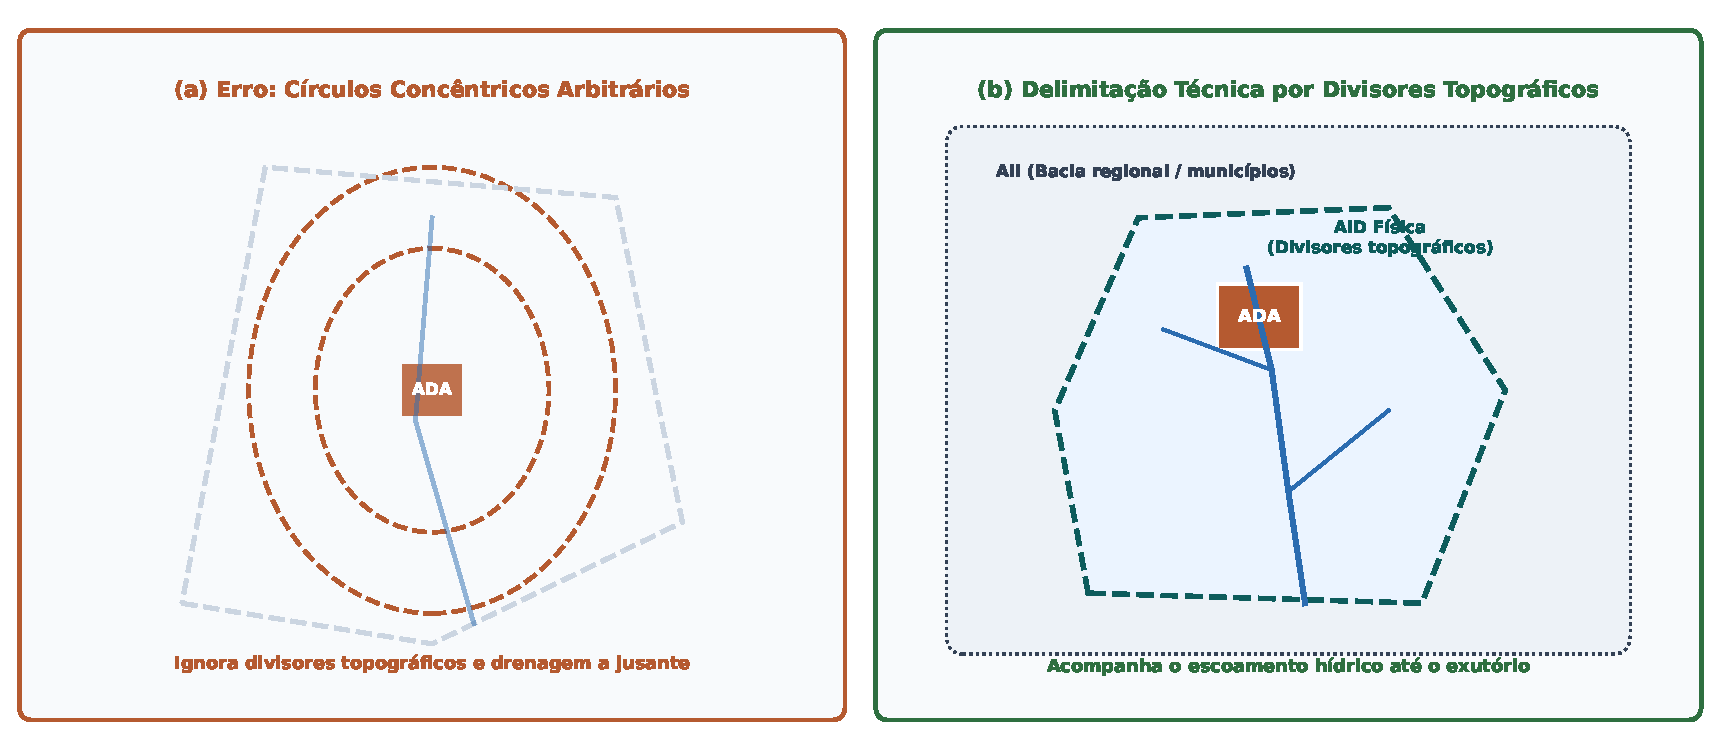
\includegraphics[width=0.96\textwidth]{figures/fig_cap05_areas_influencia.pdf}
  \caption{Delimitação técnica das Áreas de Influência (ADA, AID e AII) em bacia hidrográfica: (a) traçado circular arbitrário que ignora o escoamento e (b) delimitação física orientada pelos divisores topográficos e pela rede de drenagem a jusante da ADA. Fonte: elaboração didática CHF662 com base em Sánchez (2013).}
  \label{fig:areas_influencia}
\end{figure}

O Exemplo 5.1 quantifica a proporção espacial entre ADA, AID e AII em um empreendimento solar no Semiárido baiano.

\begin{boxExemplo}{5.1}{Delimitação Quantitativa de ADA, AID e AII em Parque Solar no Semiárido (Básico)}
  \passoEnunciado{Uma empresa propõe a instalação de uma usina solar fotovoltaica em área rural de transição semiárida na Bahia. O projeto prevê $45{,}0\text{ ha}$ ocupados pelos arranjos de painéis solares e $3{,}5\text{ ha}$ destinados à subestação, canteiro de obras e estradas internas de acesso. A microbacia hidrográfica que drena o empreendimento possui $620{,}0\text{ ha}$, e o município de inserção ocupa $48.500{,}0\text{ ha}$.}
  \passoDados{Área dos painéis $= 45{,}0\text{ ha}$; áreas de apoio e acessos $= 3{,}5\text{ ha}$; área da microbacia (AID do meio físico) $= 620{,}0\text{ ha}$; área do município (AII socioeconômica) $= 48.500{,}0\text{ ha}$.}
  \passoPedido{Calcular a Área Diretamente Afetada (ADA) total, determinar o percentual que a ADA representa em relação à AID e à AII, e justificar por que a AID do meio físico deve acompanhar os divisores da microbacia.}
  \passoMetodo{Soma das superfícies de intervenção direta para obtenção da ADA e cálculo das razões percentuais ($\text{ADA}/\text{AID} \times 100\%$ e $\text{ADA}/\text{AII} \times 100\%$), segundo os critérios espaciais de Sánchez (2013).}
  \passoContas{%
    Somando as superfícies de supressão e ocupação direta, obtém-se a ADA total e suas proporções nas áreas de influência:
    \begin{align*}
      \text{ADA} &= 45{,}0 + 3{,}5 = 48{,}5\text{ ha} \\
      \frac{\text{ADA}}{\text{AID}} \times 100\% &= \frac{48{,}5}{620{,}0} \times 100\% \approx 7{,}82\% \\
      \frac{\text{ADA}}{\text{AII}} \times 100\% &= \frac{48{,}5}{48.500{,}0} \times 100\% = 0{,}10\%.
    \end{align*}
    Quanto ao critério físico, o escoamento superficial, o carreamento de sedimentos e eventuais vazamentos de transformadores seguem a gravidade e os divisores topográficos. Um círculo fixo de $1\text{ km}$ incluiria trechos de bacias vizinhas sem conexão hídrica com o parque e deixaria de fora o exutório a jusante que receberá os sedimentos.}
  \passoResposta{$\text{ADA} = 48{,}5\text{ ha}$, correspondendo a $7{,}82\%$ da AID (microbacia) e $0{,}10\%$ da AII (município). A AID física deve coincidir com a microbacia porque os fluxos hidrossedimentológicos seguem a drenagem natural.}
  \passoVerificacao{A hierarquia espacial $\text{ADA} < \text{AID} < \text{AII}$ ($48{,}5 < 620{,}0 < 48.500{,}0\text{ ha}$) é coerente. Embora $0{,}10\%$ do município pareça pequeno na escala da AII, ocupar $7{,}82\%$ da microbacia local com superfícies compactadas altera o pico de escoamento superficial se faltarem drenagem e proteção do solo.}
\end{boxExemplo}

\subsection{Identificação, Previsão e Valoração de Impactos}

Nesta etapa, cruzam-se as ações do projeto (planejamento, implantação, operação e desativação) com os fatores ambientais descritos na linha de base. Cada impacto é caracterizado quanto à \textbf{natureza} (adverso ou benéfico), \textbf{incidência} (direto ou indireto), \textbf{abrangência} (local, regional ou estratégica), \textbf{temporalidade} (imediato, médio ou longo prazo), \textbf{duração} (temporário, permanente ou cíclico), \textbf{reversibilidade} (reversível ou irreversível) e \textbf{cumulatividade ou sinergia} com outros empreendimentos da bacia.

Quatro famílias metodológicas sustentam essa identificação e valoração conforme a complexidade do projeto. As \textbf{listagens de controle (\textit{checklists})} reúnem fatores ambientais e impactos potenciais por tipologia de obra em formato simples, descritivo ou escalar, oferecendo rapidez e padronização na triagem e no escopo, ainda que sejam estáticas e tenham dificuldade para explicitar encadeamentos indiretos. As \textbf{matrizes de interação}, com destaque para a Matriz de Leopold (Leopold et al., 1971) e suas versões ponderadas, cruzam em tabela bidimensional as ações do empreendimento (colunas) com os fatores ambientais (linhas), avaliando cada interação por sinal, magnitude e importância para hierarquizar prioridades.

Para rastrear cadeias causais complexas, empregam-se as \textbf{redes de interação (\textit{networks})}, estruturadas como grafos causa-efeito que encadeiam um impacto primário (direto) aos impactos secundários e terciários (indiretos). No Semiárido, a abertura de uma estrada sem sistema de drenagem desencadeia compactação e exposição do solo com concentração do escoamento superficial (1ª ordem), que evolui para sulcos erosivos, ravinas e carreamento de sedimentos ao riacho (2ª ordem) até assorear o açude comunitário e reduzir a oferta hídrica na estiagem (3ª ordem), encadeamento esquematizado na Figura~\ref{fig:rede_interacao}.

\begin{figure}[H]
  \centering
  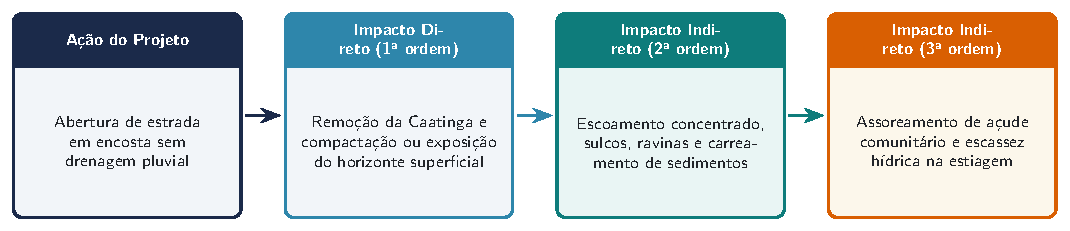
\includegraphics[width=0.95\textwidth]{figures/fig_cap05_rede_interacao.pdf}
  \caption{Rede de interação em cascata a partir da abertura de estrada sem drenagem, conectando a compactação inicial (1ª ordem) ao ravinamento (2ª ordem) e ao assoreamento de açudes a jusante (3ª ordem). Fonte: elaboração didática CHF662.}
  \label{fig:rede_interacao}
\end{figure}

Em campo, a transição da compactação inicial para o escoamento concentrado torna-se visível assim que as primeiras chuvas intensas incidem sobre a faixa exposta da via sem caixas secas ou saídas d'água, abrindo sulcos laterais que conduzem sedimentos para as drenagens próximas (Figura~\ref{fig:foto_estrada_sulco}).

\begin{figure}[H]
  \centering
  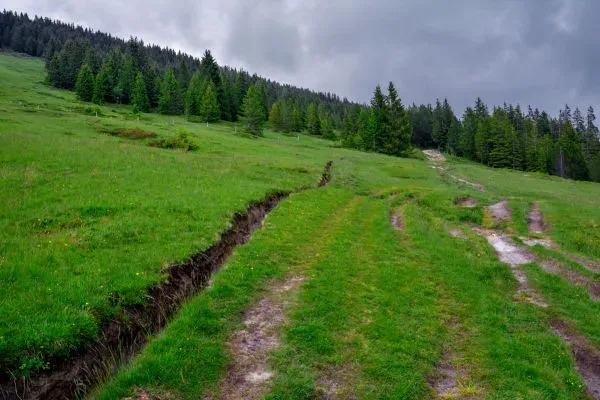
\includegraphics[width=0.68\textwidth]{figures/foto_estrada_sulco_erosivo.jpg}
  \caption{Registro de campo de escoamento concentrado e formação de sulco erosivo lateral em acesso rural sem drenagem pluvial. Fonte: acervo didático CHF662.}
  \label{fig:foto_estrada_sulco}
\end{figure}

Na quarta família metodológica, a \textbf{sobreposição de cartas (\textit{overlay}) e Sistemas de Informação Geográfica (SIG)}, derivada do método de Ian McHarg (1969), cruza camadas georreferenciadas (declividade, solos, hidrografia, APPs, remanescentes florestais e áreas urbanas) por álgebra de mapas. Essa abordagem explicita a distribuição espacial exata dos conflitos e subsidia a comparação de alternativas locacionais, dependendo da qualidade e da escala da base cartográfica adotada, tema aprofundado no Capítulo 6. A tabela a seguir sintetiza a escolha prática entre os quatro métodos.

\begin{center}
\renewcommand{\arraystretch}{1.20}
\small
\begin{tabularx}{\textwidth}{@{}p{2.7cm} >{\raggedright\arraybackslash}X >{\raggedright\arraybackslash}X p{2.7cm}@{}}
  \toprule
  \rowcolor{uefsNavy}
  \textcolor{white}{\bfseries Método} & \textcolor{white}{\bfseries Principal vantagem} & \textcolor{white}{\bfseries Principal limitação} & \textcolor{white}{\bfseries Uso ideal} \\
  \midrule
  \textbf{Checklists} & Rapidez e padronização inicial. & Estrutura estática, sem cadeias causais. & Triagem e escopo. \\
  \rowcolor{bgGray}
  \textbf{Matriz de Leopold} & Liga ações a fatores e prioriza ações críticas. & Pouca clareza para efeitos indiretos. & Síntese de EIAs e PCAs. \\
  \textbf{Redes de Interação} & Evidencia impactos indiretos e cumulativos. & Visualmente complexa em grandes projetos. & Bacias, erosão e hidrologia. \\
  \rowcolor{bgGray}
  \textbf{Sobreposição / SIG} & Localiza conflitos e compara traçados. & Depende da escala e qualidade dos mapas. & Traçados e zoneamentos. \\
  \bottomrule
\end{tabularx}
\end{center}

\subsection{Matriz de Leopold Ponderada: Magnitude, Importância e Balanço}

Na adaptação ponderada da Matriz de Leopold (Leopold et al., 1971), cada célula $(i, j)$ com interação efetiva entre o \textbf{fator ambiental $i$} (linha) e a \textbf{ação $j$} (coluna) recebe três parâmetros. O \textbf{sinal ($s_{ij} \in \{-1, +1\}$)} assume $-1$ para impacto adverso e $+1$ para impacto benéfico, registrando-se $0$ quando a interação é inexistente. A \textbf{magnitude ($M_{ij} \in \{1, \dots, 10\}$)} mede a intensidade e extensão física da alteração sobre o fator, enquanto a \textbf{importância ($I_{ij} \in \{1, \dots, 10\}$)} expressa a relevância ecológica, funcional, social ou legal do receptor atingido, atingindo notas máximas em nascentes, espécies ameaçadas ou comunidades tradicionais.

\begin{boxFormula}[Equações da Matriz de Leopold Ponderada]
\begin{align*}
  P_{ij} &= s_{ij} \cdot \left(M_{ij} \times I_{ij}\right), \qquad P_{ij} \in [-100, +100] \\[4pt]
  T_j &= \sum_{i=1}^{m} P_{ij} \qquad \text{(total da coluna } j \text{ sobre os } m \text{ fatores)} \\[4pt]
  F_i &= \sum_{j=1}^{n} P_{ij} \qquad \text{(total da linha } i \text{ sob as } n \text{ ações)} \\[4pt]
  B &= \sum_{i=1}^{m}\sum_{j=1}^{n} P_{ij} = \sum_{j=1}^{n} T_j = \sum_{i=1}^{m} F_i \\[4pt]
  \Sigma^{-} &= \sum_{P_{ij}<0} P_{ij}, \qquad \Sigma^{+} = \sum_{P_{ij}>0} P_{ij}
\end{align*}
Nessas equações, $P_{ij}$ é a pontuação celular, $T_j$ mede o saldo da ação $j$, $F_i$ acumula a pressão sobre o fator $i$, $B$ é o balanço líquido global, $\Sigma^{-}$ reúne a carga adversa total e $\Sigma^{+}$ soma a carga benéfica total.
\end{boxFormula}

Para acompanhar o cálculo em escala reduzida, considere uma mini-matriz com duas ações ($A_1$: supressão vegetal em encosta; $A_2$: contratação de mão de obra local) e dois fatores ($F_1$: solo e suscetibilidade erosiva; $F_2$: renda familiar). Na célula $(F_1, A_1)$, a supressão gera dano severo ($s=-1$, $M=8$, $I=9$), resultando em $P_{11} = -72$, enquanto em $(F_2, A_1)$ o pagamento temporário pela limpeza produz efeito positivo discreto ($s=+1$, $M=2$, $I=3$), com $P_{21} = +6$. A ação $A_2$ não altera fisicamente o solo ($P_{12} = 0$), mas eleva a renda local ($s=+1$, $M=6$, $I=7$), gerando $P_{22} = +42$. Somando colunas e linhas, tem-se $T_1 = -66$, $T_2 = +42$, $F_1 = -72$, $F_2 = +48$, carga adversa $\Sigma^{-} = -72$, carga benéfica $\Sigma^{+} = +48$ e balanço $B = -24$. A estrutura operacional dessa matriz em planilha eletrônica está representada na Figura~\ref{fig:matriz_leopold_excel}.

\begin{figure}[H]
  \centering
  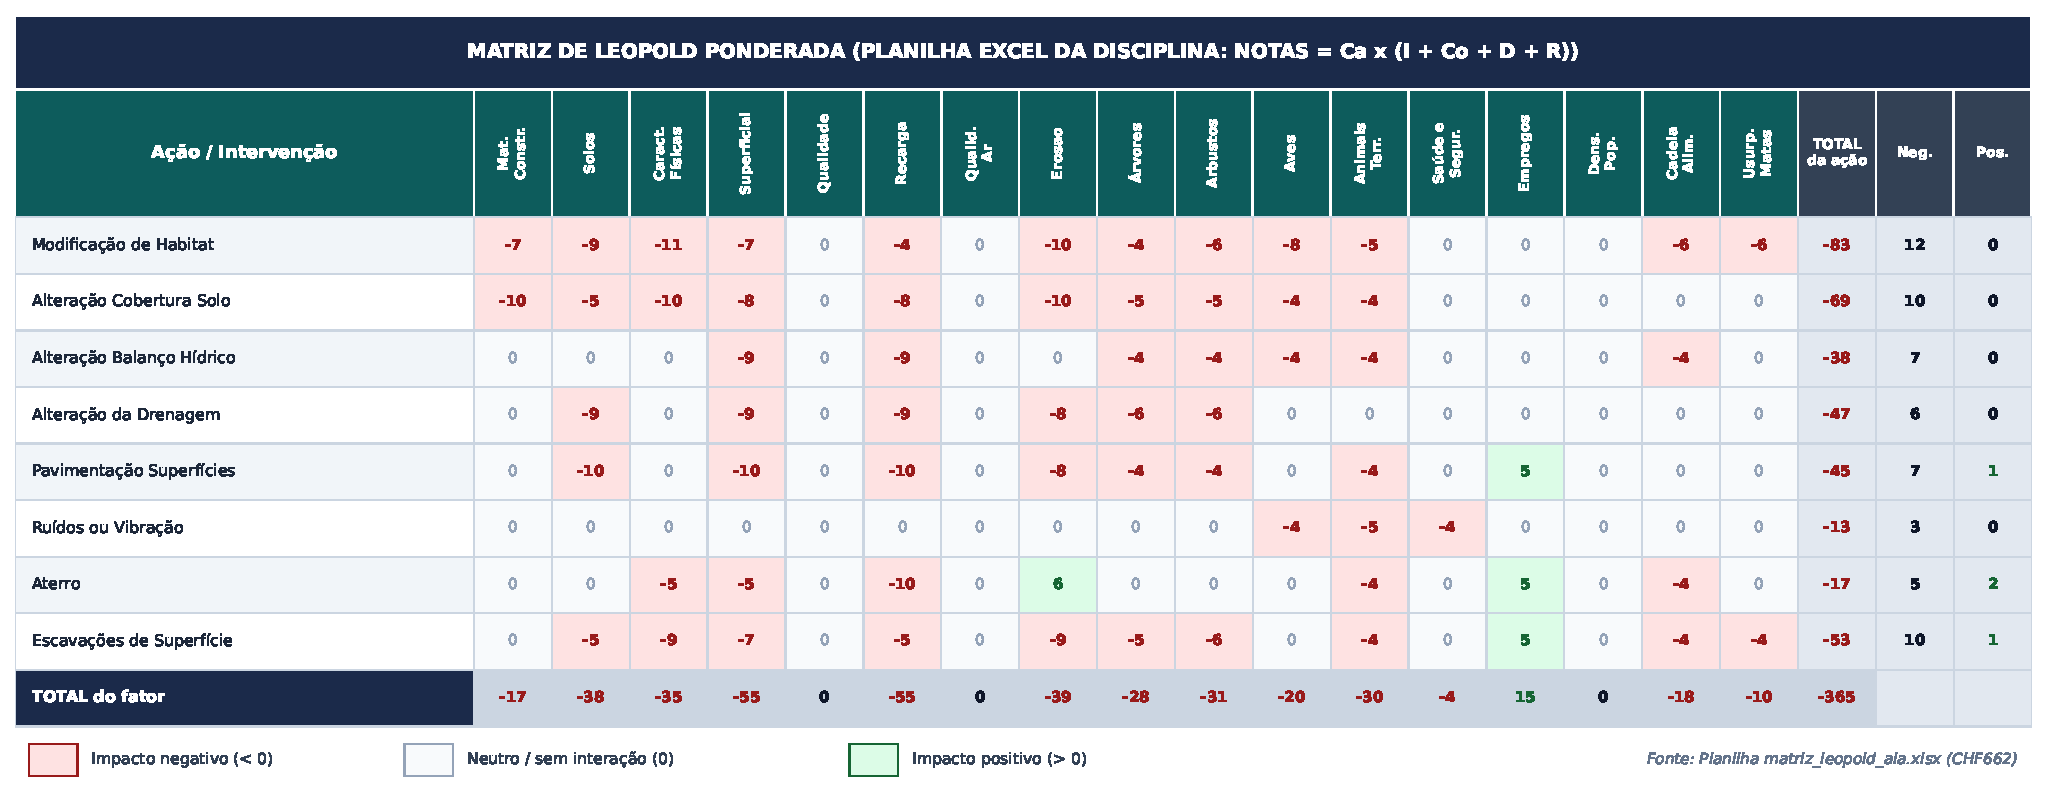
\includegraphics[width=0.98\textwidth]{figures/fig_cap05_matriz_leopold_excel.pdf}
  \caption{Matriz de Leopold Ponderada na planilha eletrônica da disciplina, destacando impactos adversos em vermelho, benéficos em verde e os totais por ação e fator ambiental. Fonte: planilha didática \texttt{matriz\_leopold\_aia.xlsx} (CHF662).}
  \label{fig:matriz_leopold_excel}
\end{figure}

O Exemplo 5.2 aplica esse equacionamento completo à avaliação de um parque eólico na Caatinga baiana.

\begin{boxExemplo}{5.2}{Matriz de Leopold Ponderada em Parque Eólico na Caatinga (Básico e Intermediário)}
  \passoEnunciado{Durante a AIA de um parque eólico no Semiárido baiano, a equipe técnica estruturou uma matriz cruzando três ações ($A_1$: supressão vegetal e abertura de acessos; $A_2$: escavação e concretagem das fundações das torres; $A_3$: operação dos aerogeradores e contratação de serviços locais) com quatro fatores ambientais ($F_1$: solo e processos erosivos; $F_2$: fauna e avifauna; $F_3$: qualidade da água superficial; $F_4$: emprego e renda local).}
  \passoDados{Avaliações $(s, M, I)$ atribuídas após vistorias de campo e linha de base: em $F_1$ (Solo/Erosão), $A_1 = (-, 8, 9)$, $A_2 = (-, 6, 8)$ e $A_3 = 0$; em $F_2$ (Fauna/Avifauna), $A_1 = (-, 7, 8)$, $A_2 = (-, 3, 5)$ e $A_3 = (-, 5, 9)$; em $F_3$ (Qualidade da água), $A_1 = (-, 5, 7)$, $A_2 = (-, 4, 7)$ e $A_3 = 0$; em $F_4$ (Emprego/Renda), $A_1 = (+, 3, 5)$, $A_2 = (+, 4, 5)$ e $A_3 = (+, 7, 8)$.}
  \passoPedido{Calcular todas as pontuações celulares $P_{ij}$, os totais por ação ($T_j$), os totais por fator ($F_i$), a carga adversa ($\Sigma^{-}$), a carga benéfica ($\Sigma^{+}$) e o balanço líquido ($B$), identificando a ação mais crítica e o fator mais impactado.}
  \passoMetodo{Aplicação das equações da Matriz de Leopold Ponderada ($P_{ij} = s_{ij} \cdot M_{ij} \cdot I_{ij}$), com verificação cruzada pela identidade $\sum T_j = \sum F_i = B$.}
  \passoContas{%
    Calculando cada célula por linha: em $F_1$, $P_{11} = -72$, $P_{12} = -48$ e $P_{13} = 0$; em $F_2$, $P_{21} = -56$, $P_{22} = -15$ e $P_{23} = -45$; em $F_3$, $P_{31} = -35$, $P_{32} = -28$ e $P_{33} = 0$; e em $F_4$, $P_{41} = +15$, $P_{42} = +20$ e $P_{43} = +56$. Os valores consolidam-se na matriz a seguir:
    \begin{center}
    \renewcommand{\arraystretch}{1.15}
    \small
    \begin{tabularx}{0.96\linewidth}{@{}X r r r r@{}}
      \toprule
      \textbf{Fator Ambiental} & \textbf{$A_1$ (Acessos)} & \textbf{$A_2$ (Fundações)} & \textbf{$A_3$ (Operação)} & \textbf{Total $F_i$} \\
      \midrule
      $F_1$, Solo / Erosão & $-72$ & $-48$ & $0$ & $\mathbf{-120}$ \\
      $F_2$, Fauna / Avifauna & $-56$ & $-15$ & $-45$ & $\mathbf{-116}$ \\
      $F_3$, Qualidade da água & $-35$ & $-28$ & $0$ & $\mathbf{-63}$ \\
      $F_4$, Emprego / Renda & $+15$ & $+20$ & $+56$ & $\mathbf{+91}$ \\
      \midrule
      \textbf{Total da Ação ($T_j$)} & $\mathbf{-148}$ & $\mathbf{-71}$ & $\mathbf{+11}$ & $\mathbf{B = -208}$ \\
      \bottomrule
    \end{tabularx}
    \end{center}
    Conferindo as somas marginais e separando as cargas adversa e benéfica:
    \begin{align*}
      \sum F_i &= (-120) + (-116) + (-63) + 91 = -208, \\
      \sum T_j &= (-148) + (-71) + 11 = -208, \\
      \Sigma^{-} &= -72 - 48 - 56 - 15 - 45 - 35 - 28 = -299, \\
      \Sigma^{+} &= +15 + 20 + 56 = +91.
    \end{align*}}
  \passoResposta{A ação mais impactante negativamente é $A_1$ (supressão e acessos, $T_1 = -148$) e o fator mais vulnerável é $F_1$ (solo/erosão, $F_1 = -120$), seguido de $F_2$ (fauna/avifauna, $F_2 = -116$). A carga adversa vale $\Sigma^{-} = -299$, a benéfica vale $\Sigma^{+} = +91$ e o balanço líquido fecha em $B = -208$.}
  \passoVerificacao{A igualdade $\sum F_i = \sum T_j = \Sigma^{-} + \Sigma^{+} = -208$ confirma a exatidão aritmética. Mesmo com $T_3 = +11$ na operação, a célula $P_{23} = -45$ (colisão de avifauna, com importância $I = 9$) exige monitoramento e desligamento preventivo para espécies como a arara-azul-de-lear na região de Canudos, jamais sendo anulada pelos $+56$ pontos de renda.}
\end{boxExemplo}

A interpretação isolada do saldo líquido $B$ costuma induzir erros graves na tomada de decisão, conforme detalhado no alerta a seguir.

\begin{boxErro}[Erro 2: Somar Benefícios Econômicos com Danos Ecológicos na Matriz]
  \textbf{Equívoco frequente:} Concluir que um empreendimento é ambientalmente viável porque a soma algébrica $B = \Sigma^{+} + \Sigma^{-}$ ficou positiva ou próxima de zero (por exemplo, $+80$ em arrecadação contra $-75$ em destruição de nascente).\par
  \textbf{Correção técnica:} A pontuação da Matriz de Leopold é semiquantitativa e reúne dimensões incomensuráveis. Empregos temporários não evitam o assoreamento de mananciais nem compensam a extinção local de fauna. Por isso, deve-se reportar $\Sigma^{-}$ e $\Sigma^{+}$ separadamente, destacando toda célula adversa de alta importância ($I \ge 8$) ou irreversível para vinculá-la a medidas concretas de mitigação.
\end{boxErro}

\subsection{Prognóstico Ambiental e Efeitos Cumulativos}

O prognóstico projeta a evolução futura da qualidade ambiental por meio de dois cenários comparativos obrigatórios com o mesmo horizonte temporal. O \textbf{cenário sem projeto (alternativa zero)} retrata a trajetória provável da bacia na ausência da obra, incorporando tendências já em curso como expansão urbana, sobrepastejo, variações climáticas ou regeneração natural. O \textbf{cenário com projeto} projeta a trajetória com o empreendimento em dois estágios: primeiro sem medidas mitigadoras, para dimensionar o risco potencial, e em seguida com os controles propostos, revelando o impacto residual. O impacto real atribuível ao projeto corresponde à diferença dinâmica entre a trajetória futura com o projeto e a trajetória futura sem o projeto.

Essa projeção deve considerar também os \textbf{impactos cumulativos}, que emergem quando pressões de diferentes empreendimentos convergem sobre o mesmo receptor. Estradas de parques eólicos vizinhos podem direcionar enxurradas para o mesmo riacho, enquanto captações distintas afetam a disponibilidade hídrica do mesmo trecho fluvial, exigindo definir explicitamente o receptor, a área de acumulação e o período analisado. O Exemplo 5.3 mostra como comparar alternativas locacionais no prognóstico por meio de critérios ponderados.

\begin{boxExemplo}{5.3}{Prognóstico e Seleção Multicritério de Alternativas Locacionais (Intermediário)}
  \passoEnunciado{No estudo de duplicação de uma rodovia estadual na Bahia, o EIA comparou duas alternativas locacionais diante do cenário sem projeto: o \textbf{Traçado A} (mais curto, atravessando uma APP de nascente e um fragmento contínuo de Caatinga) e o \textbf{Traçado B} ($1{,}2\text{ km}$ mais extenso, contornando a APP por áreas já antropizadas de pastagem).}
  \passoDados{Quatro critérios ponderados (soma dos pesos $= 1{,}00$) em escala de \textbf{severidade adversa} de $0$ (nenhum dano) a $10$ (dano máximo): $C_1$, supressão de APP e vegetação nativa ($w_1 = 0{,}35$; A $= 9$, B $= 3$); $C_2$, risco erosivo e assoreamento ($w_2 = 0{,}30$; A $= 8$, B $= 4$); $C_3$, fragmentação e atropelamento de fauna ($w_3 = 0{,}20$; A $= 8$, B $= 4$); $C_4$, custo e extensão adicional ($w_4 = 0{,}15$; A $= 4$, B $= 7$).}
  \passoPedido{Calcular o Índice de Impacto Adverso Ponderado ($I_{\text{adv}}$) de cada alternativa, determinar a redução percentual do índice ao optar pelo melhor traçado e identificar o degrau da Hierarquia de Mitigação correspondente.}
  \passoMetodo{Cálculo da média ponderada $I_{\text{adv}} = \sum_{k=1}^{4} w_k \cdot C_k$ e da variação relativa $(I_A - I_B)/I_A \times 100\%$.}
  \passoContas{%
    Os pesos somam $0{,}35 + 0{,}30 + 0{,}20 + 0{,}15 = 1{,}00$. Calculando os índices ponderados e a redução relativa de severidade:
    \begin{align*}
      I_A &= (0{,}35 \times 9) + (0{,}30 \times 8) + (0{,}20 \times 8) + (0{,}15 \times 4) \\
          &= 3{,}15 + 2{,}40 + 1{,}60 + 0{,}60 = 7{,}75 \\
      I_B &= (0{,}35 \times 3) + (0{,}30 \times 4) + (0{,}20 \times 4) + (0{,}15 \times 7) \\
          &= 1{,}05 + 1{,}20 + 0{,}80 + 1{,}05 = 4{,}10 \\
      \text{Redução} &= \frac{7{,}75 - 4{,}10}{7{,}75} \times 100\% = \frac{3{,}65}{7{,}75} \times 100\% \approx 47{,}10\%.
    \end{align*}}
  \passoResposta{O Traçado B é superior ($I_B = 4{,}10$ contra $I_A = 7{,}75$), reduzindo em $47{,}10\%$ a severidade adversa global. Essa escolha representa o 1º degrau da Hierarquia de Mitigação (\textbf{Evitar}), por alternativa locacional.}
  \passoVerificacao{Como a escala mede severidade adversa, o menor valor indica melhor desempenho. Apesar do maior custo inicial no critério $C_4$ ($7$ contra $4$), o Traçado B evita intervenções em APP, obras emergenciais contra erosão e passivos de compensação.}
\end{boxExemplo}

\subsection{Hierarquia de Mitigação, Medidas Mitigadoras e Compensatórias}

Diante de impactos adversos previstos, a tomada de decisão obedece a uma ordem estrita de prioridade técnica conhecida como \textbf{Hierarquia de Mitigação}, representada no Painel (b) da Figura~\ref{fig:aia_mitigacao}. No \textbf{1º degrau, Evitar (prevenção na origem)}, ajustam-se localização, traçado, cronograma ou tecnologia para impedir que o impacto ocorra, sendo o nível de maior eficácia ecológica. Quando a prevenção integral é inviável, aplica-se o \textbf{2º degrau, Minimizar}, utilizando controles de engenharia e manejo (como bacias de contenção de sedimentos, supressão seletiva e controle de poeira) para abater magnitude, duração ou extensão do dano.

Nas áreas afetadas temporariamente durante a obra, como canteiros, taludes de corte e áreas de empréstimo, atua-se no \textbf{3º degrau, Recuperar ou Reabilitar (\textit{in situ})}, restabelecendo as funções do solo, da drenagem e da cobertura vegetal mediante Plano de Recuperação de Áreas Degradadas (PRAD) e bioengenharia. Somente para o dano inevitável que persiste após esses três degraus, denominado \textbf{impacto residual}, recorre-se ao \textbf{4º degrau, Compensar}, por meio de apoio a Unidades de Conservação (art. 36 da Lei nº 9.985/2000, SNUC), reposição florestal equivalente ou superior e programas comunitários. De modo paralelo, impactos benéficos recebem \textbf{medidas potencializadoras}, como capacitação profissional prévia para ampliar a contratação de moradores locais.

O Exemplo 5.4 demonstra o abatimento sequencial (em cascata) ao longo dos quatro degraus da Hierarquia de Mitigação.

\begin{boxExemplo}{5.4}{Aplicação Sequencial da Hierarquia de Mitigação em Loteamento Periurbano (Intermediário e Avançado)}
  \passoEnunciado{O anteprojeto de um loteamento periurbano previa a supressão de $12{,}0\text{ ha}$ de vegetação nativa e um aporte de $480{,}0\text{ t/ano}$ de sedimentos para um riacho a jusante. Após revisão técnica, aplicaram-se sequencialmente os quatro degraus da Hierarquia de Mitigação.}
  \passoDados{No degrau \textbf{Evitar}, a exclusão de quadras em encostas íngremes evita $45\%$ da supressão e $45\%$ do aporte de sedimentos. No degrau \textbf{Minimizar}, o corte seletivo poupa $1{,}6\text{ ha}$ e bacias de contenção retêm $60\%$ do sedimento restante. No degrau \textbf{Recuperar}, a bioengenharia recupera $2{,}0\text{ ha}$ temporários e retém $75\%$ do sedimento remanescente. No degrau \textbf{Compensar}, exige-se reposição na razão $2{:}1$ sobre a perda permanente residual.}
  \passoPedido{Calcular o saldo remanescente de vegetação afetada e de sedimentos em cada degrau, o abatimento percentual acumulado de sedimentos e a área de compensação ecológica no 4º degrau.}
  \passoMetodo{Abatimento em cascata sobre o saldo remanescente de cada etapa, evitando somar percentuais diretamente sobre a carga inicial.}
  \passoContas{%
    Para a trajetória da supressão vegetal (em $\text{ha}$) e do aporte de sedimentos (em $\text{t/ano}$), aplicam-se os abatimentos etapa a etapa:
    \begin{align*}
      \text{Vegetação após Evitar} &= 12{,}0 - (0{,}45 \times 12{,}0) = 12{,}0 - 5{,}4 = 6{,}6\text{ ha} \\
      \text{após Minimizar} &= 6{,}6 - 1{,}6 = 5{,}0\text{ ha} \\
      \text{após Recuperar (residual)} &= 5{,}0 - 2{,}0 = 3{,}0\text{ ha} \\
      \text{Área a Compensar (}2{:}1\text{)} &= 2 \times 3{,}0 = 6{,}0\text{ ha}
    \end{align*}
    \begin{align*}
      \text{Sedimentos após Evitar} &= 480{,}0 - (0{,}45 \times 480{,}0) = 264{,}0\text{ t/ano} \\
      \text{após Minimizar} &= 264{,}0 - (0{,}60 \times 264{,}0) = 105{,}6\text{ t/ano} \\
      \text{após Recuperar (residual)} &= 105{,}6 - (0{,}75 \times 105{,}6) = 26{,}4\text{ t/ano} \\
      \text{Abatimento acumulado} &= \frac{480{,}0 - 26{,}4}{480{,}0} \times 100\% = 94{,}50\%.
    \end{align*}}
  \passoResposta{O impacto residual permanente reduz-se a $3{,}0\text{ ha}$ de vegetação (exigindo $6{,}0\text{ ha}$ de compensação na razão $2{:}1$) e a $26{,}4\text{ t/ano}$ de sedimentos (abatimento total de $94{,}50\%$).}
  \passoVerificacao{Pelo produto em cascata, $480{,}0 \times 0{,}55 \times 0{,}40 \times 0{,}25 = 26{,}4\text{ t/ano}$. Sem seguir a hierarquia, tentar compensar os $12{,}0\text{ ha}$ iniciais exigiria $24{,}0\text{ ha}$ de reposição e manteria o riacho assoreado com $480\text{ t/ano}$ de sedimentos.}
\end{boxExemplo}

Propor compensação financeira antes de esgotar alternativas locacionais e medidas de engenharia viola diretamente a Hierarquia de Mitigação, como alerta o quadro a seguir.

\begin{boxErro}[Erro 3: Inverter a Hierarquia de Mitigação ao Priorizar a Compensação]
  \textbf{Equívoco frequente:} Propor diretamente compensação financeira ou plantio em outro município para suprimir uma APP ou fragmento florestal sem avaliar alternativas de traçado ou tecnologia que evitassem a perda.\par
  \textbf{Correção técnica:} A compensação ocupa o \textbf{4º e último degrau} da hierarquia, destinando-se exclusivamente ao impacto residual que permanece após esgotadas as etapas de evitar, minimizar e recuperar no local.
\end{boxErro}

\subsection{Plano Básico Ambiental (PBA) e Monitoramento Pós-Implantação}

Na etapa decisória, o órgão ambiental emite parecer técnico pelo deferimento com condicionantes ou pelo indeferimento das licenças (Licença Prévia, Licença de Instalação e Licença de Operação). Os compromissos assumidos no EIA convertem-se em projetos executivos detalhados no \textbf{Plano Básico Ambiental (PBA)}, que estrutura programas de controle de erosão, monitoramento da qualidade da água, resgate de fauna, educação ambiental e PRAD. Cada programa necessita de condição inicial documentada, meta verificável, frequência de amostragem e responsável técnico.

O \textbf{monitoramento pós-implantação} fecha o ciclo da AIA ao confrontar os indicadores medidos em operação com os valores da linha de base e interpretar desvios junto aos registros de chuva e manutenção. Caso um indicador ultrapasse o limite da condicionante ambiental, aciona-se a \textbf{gestão adaptativa} para corrigir imediatamente os dispositivos de controle em campo.

% ============================================================================
% ETAPA 4 — ESTUDO DE CASO AVANÇADO (EXEMPLO 5.5)
% ============================================================================
\etapa{4}{Aplicação Integrada: Auditoria de Monitoramento no PBA}

A verificação quantitativa de desempenho durante a obra exige descontar a condição natural registrada na linha de base antes de calcular a eficiência das medidas de controle, evitando subestimar ou superestimar o abatimento real obtido em campo, como demonstrado no Exemplo 5.5.

\begin{boxExemplo}{5.5}{Auditoria de Eficiência no Monitoramento Pós-Implantação do PBA (Avançado)}
  \passoEnunciado{Durante a construção de uma barragem de regularização hídrica no rio Jacuípe (Bahia), a linha de base registrou turbidez média de $18{,}0\text{ NTU}$ a jusante em estiagem. Na terraplenagem inicial sem controle, a turbidez subiu para $112{,}0\text{ NTU}$. Após a instalação de cortinas de siltagem e diques do PBA, o monitoramento mediu $33{,}0\text{ NTU}$. A condicionante da Licença de Instalação fixava limite máximo de $40{,}0\text{ NTU}$.}
  \passoDados{Linha de base $T_0 = 18{,}0\text{ NTU}$; turbidez sem mitigação $T_{\text{sem}} = 112{,}0\text{ NTU}$; turbidez com PBA $T_{\text{com}} = 33{,}0\text{ NTU}$; limite legal $T_{\max} = 40{,}0\text{ NTU}$.}
  \passoPedido{Calcular o acréscimo de turbidez atribuível à obra sem mitigação, o acréscimo residual após o PBA, a eficiência percentual de abatimento da carga antrópica e emitir parecer técnico sobre o atendimento à condicionante.}
  \passoMetodo{Cálculo da anomalia acima da linha de base ($\Delta T = T - T_0$) e da eficiência de abatimento incremental $E_f = \frac{\Delta T_{\text{sem}} - \Delta T_{\text{com}}}{\Delta T_{\text{sem}}} \times 100\%$.}
  \passoContas{%
    Descontando a turbidez natural $T_0$ da linha de base, calculam-se os acréscimos e a eficiência do PBA:
    \begin{align*}
      \Delta T_{\text{sem}} &= 112{,}0 - 18{,}0 = 94{,}0\text{ NTU} \\
      \Delta T_{\text{com}} &= 33{,}0 - 18{,}0 = 15{,}0\text{ NTU} \\
      \Delta T_{\text{abatida}} &= 94{,}0 - 15{,}0 = 79{,}0\text{ NTU} \\
      E_f &= \frac{79{,}0}{94{,}0} \times 100\% \approx 84{,}04\%.
    \end{align*}
    Como $33{,}0\text{ NTU} \le 40{,}0\text{ NTU}$, a condicionante da Licença de Instalação está atendida com folga de $7{,}0\text{ NTU}$.}
  \passoResposta{O acréscimo sem controle foi de $94{,}0\text{ NTU}$, reduzido para $15{,}0\text{ NTU}$ residuais com eficiência de abatimento de $84{,}04\%$. A condicionante de $40{,}0\text{ NTU}$ está atendida, mantendo-se o monitoramento contínuo na estação chuvosa.}
  \passoVerificacao{Descontar $T_0 = 18{,}0\text{ NTU}$ no denominador é indispensável porque o controle ambiental visa abater o acréscimo gerado pela obra sobre o fundo natural do rio; sem esse desconto, o cálculo subestimaria a eficiência real ($79/112 = 70{,}54\%$).}
\end{boxExemplo}

% ============================================================================
% ETAPA 5 — ERRO 4 E MATERIAIS AUDIOVISUAIS DE APOIO
% ============================================================================
\etapa{5}{Armadilha Conceitual e Materiais Audiovisuais de Apoio}

Mesmo quando um estudo adota equações corretas na matriz de impacto ou no monitoramento do PBA, uma delimitação espacial mal fundamentada compromete toda a amostragem dos meios físico, biótico e socioeconômico.

\begin{boxErro}[Erro 4: Delimitar ADA, AID e AII como Círculos Concêntricos Arbitrários]
  \textbf{Equívoco frequente:} Traçar raios fixos de $500\text{ m}$ (AID) e $5\text{ km}$ (AII) no mapa sem considerar divisores de bacia, direção dos ventos, rotas de fauna ou malha viária.\par
  \textbf{Correção técnica:} Processos ambientais propagam-se segundo fluxos físicos e sociais anisotrópicos. Um efluente lançado num riacho percorre quilômetros a jusante pelo talvegue, mas permanece ausente a $200\text{ m}$ além do divisor topográfico. Delimite a AID física pela microbacia drenada, a AID biótica pelos habitats conectados e a AII pela rede territorial e municipal afetada.
\end{boxErro}

Para consolidar o entendimento sobre degradação ambiental, papel preventivo da AIA e estruturação de EIA/RIMA, assista às videoaulas selecionadas na página da disciplina: \textit{O papel da Avaliação de Impacto Ambiental na gestão ambiental} (\url{https://www.youtube.com/watch?v=oDceh9hvPc8}), \textit{EIA-RIMA, Conceitos e Definições de Impactos Ambientais} (\url{https://www.youtube.com/watch?v=m8rg8SnhSfQ}) e \textit{Degradação Ambiental} (\url{https://www.youtube.com/watch?v=5EFxN7jGob8}), que articulam diagnóstico, prognóstico e medidas mitigadoras no licenciamento brasileiro.

% ============================================================================
% ETAPA 6 — EXERCÍCIOS DE FIXAÇÃO (15 EXERCÍCIOS: 5 BÁSICOS, 5 INTERM., 5 OBJ.)
% ============================================================================
\etapa{6}{Exercícios de Fixação}

\subsection*{Nível 1: Básico (Conceitos, Etapas e Cálculos Fundamentais)}

\begin{enumerate}[leftmargin=1.8em, itemsep=4pt]
  \item Explique, com base em Sánchez (2013), qual é o papel preventivo da Avaliação de Impacto Ambiental (AIA) e por que sua inserção tardia, após a definição do projeto de engenharia, compromete sua eficácia no planejamento ambiental.
  \espacoResolucao[2.0cm]

  \item Em uma matriz de interação ponderada adaptada de Leopold, uma atividade de terraplenagem apresentou três interações relevantes: solo e erosão $(-, M=7, I=8)$; qualidade do ar por poeira $(-, M=4, I=6)$; e contratação temporária de operadores locais $(+, M=6, I=5)$. Calcule a pontuação $P_{ij}$ de cada célula, a carga adversa ($\Sigma^{-}$), a carga benéfica ($\Sigma^{+}$) e o total $T_j$ dessa ação.
  \espacoResolucao[2.2cm]

  \item Diferencie claramente as etapas de \textbf{triagem (\textit{screening})} e \textbf{definição de escopo (\textit{scoping})}, indicando qual documento oficial formaliza o resultado da definição de escopo no licenciamento ambiental brasileiro.
  \espacoResolucao[2.0cm]

  \item Defina \textbf{ADA}, \textbf{AID} e \textbf{AII} e dê um exemplo concreto de cada uma para a implantação de um aterro sanitário regional no interior da Bahia.
  \espacoResolucao[2.1cm]

  \item Compare as quatro famílias de métodos de identificação de impactos (\textit{checklists}, Matriz de Leopold, redes de interação e sobreposição de cartas em SIG), indicando uma vantagem específica de cada método.
  \espacoResolucao[2.2cm]
\end{enumerate}

\subsection*{Nível 2: Intermediário (Aplicação Quantitativa e Análise Técnica)}

\begin{enumerate}[leftmargin=1.8em, itemsep=4pt, resume]
  \item Um empreendimento de extração de areia em planície fluvial foi avaliado por meio de uma matriz ponderada $3 \times 3$, com as ações $A_1$ (dragagem no leito), $A_2$ (abertura de pátio e estrada de acesso) e $A_3$ (comercialização e geração de empregos) e os fatores $F_1$ (estabilidade das margens e do leito), $F_2$ (turbidez e biota aquática) e $F_3$ (renda e arrecadação municipal):
  \begin{itemize}[leftmargin=1.4em, itemsep=1pt]
    \item $F_1$: $A_1=(-, 9, 9)$; $A_2=(-, 5, 7)$; $A_3=0$.
    \item $F_2$: $A_1=(-, 8, 8)$; $A_2=(-, 4, 6)$; $A_3=0$.
    \item $F_3$: $A_1=(+, 3, 4)$; $A_2=(+, 2, 4)$; $A_3=(+, 6, 6)$.
  \end{itemize}
  Calcule todas as células $P_{ij}$, os totais $T_j$ e $F_i$, $\Sigma^{-}$, $\Sigma^{+}$ e o balanço $B$. Identifique a ação mais degradadora e o fator mais crítico.
  \espacoResolucao[3.2cm]

  \item Um projeto agroindustrial previa inicialmente suprimir $20{,}0\text{ ha}$ de vegetação nativa. Aplicando a Hierarquia de Mitigação, a realocação do galpão evitou $35\%$ da supressão inicial; o ajuste das vias internas minimizou $20\%$ da área restante; e a restauração de áreas temporárias recuperou $2{,}4\text{ ha}$. Sabendo que o órgão licenciador determinou compensação na razão $3{:}1$ sobre o impacto permanente residual, calcule a área remanescente em cada degrau e a área total a ser compensada.
  \espacoResolucao[2.8cm]

  \item Na escolha tecnológica para uma Estação de Tratamento de Efluentes (ETE), duas opções ($E_1$ e $E_2$) foram avaliadas em escala de \textbf{desempenho ambiental positivo} ($0$ = péssimo; $10$ = excelente) sob quatro critérios ponderados: eficiência de remoção de carga orgânica ($w_1 = 0{,}35$: $E_1=6$, $E_2=9$), controle de odores ($w_2 = 0{,}30$: $E_1=5$, $E_2=8$), possibilidade de reúso agrícola no Semiárido ($w_3 = 0{,}20$: $E_1=7$, $E_2=8$) e menor custo de implantação ($w_4 = 0{,}15$: $E_1=9$, $E_2=6$). Calcule a nota ponderada de cada alternativa e justifique a escolha técnica.
  \espacoResolucao[2.6cm]

  \item Desenhe ou descreva textualmente uma \textbf{rede de interação} de três níveis (impacto primário $\to$ secundário $\to$ terciário) desencadeada pela abertura de vias de acesso sem drenagem em encosta declivosa da Caatinga, associando ao menos uma medida preventiva e uma medida corretiva do PBA para interromper a cascata.
  \espacoResolucao[2.4cm]

  \item No monitoramento do PBA de uma obra rodoviária, a linha de base de Sólidos Suspensos Totais (SST) em um riacho era de $25{,}0\text{ mg/L}$. Durante a escavação sem bacias de decantação, o valor atingiu $145{,}0\text{ mg/L}$. Após a implantação das bacias previstas no PBA, a concentração caiu para $43{,}0\text{ mg/L}$. Calcule o acréscimo sem controle, o acréscimo residual e a eficiência percentual de abatimento da carga antrópica.
  \espacoResolucao[2.4cm]
\end{enumerate}

\subsection*{Nível 3: Questões Objetivas de Fixação (A a E)}

\begin{enumerate}[leftmargin=1.8em, itemsep=5pt, resume]
  \item \textbf{[Autoral, CHF662]} No processo de Avaliação de Impacto Ambiental, o prognóstico compara o cenário com projeto ao cenário sem projeto (alternativa zero). Assinale a alternativa que interpreta corretamente o conceito de \textbf{cenário sem projeto}:
  \begin{alternativas}
    \item Representa a manutenção estática e imutável das condições atuais medidas na linha de base, sem qualquer variação futura.
    \item Projeta a evolução futura provável do ambiente na ausência do empreendimento, incorporando tendências climáticas, ecológicas e de uso da terra já em curso.
    \item Equivale ao cenário com projeto após a aplicação integral das medidas compensatórias previstas no PBA.
    \item É exigido apenas quando o empreendedor decide abandonar a obra antes da emissão da Licença Prévia.
    \item Dispensa a realização do diagnóstico ambiental da linha de base nos meios físico e biótico.
  \end{alternativas}
  \espacoResolucao[1.2cm]

  \item \textbf{[Autoral, CHF662]} Assinale a alternativa que apresenta na ordem correta, da maior para a menor prioridade técnica e ecológica, os degraus da \textbf{Hierarquia de Mitigação}:
  \begin{alternativas}
    \item Compensar $\to$ Recuperar $\to$ Minimizar $\to$ Evitar.
    \item Minimizar $\to$ Evitar $\to$ Compensar $\to$ Recuperar.
    \item Evitar $\to$ Recuperar $\to$ Minimizar $\to$ Compensar.
    \item Evitar $\to$ Minimizar $\to$ Recuperar $\to$ Compensar.
    \item Monitorar $\to$ Compensar $\to$ Evitar $\to$ Minimizar.
  \end{alternativas}
  \espacoResolucao[1.2cm]

  \item \textbf{[Autoral, CHF662]} Em uma Matriz de Leopold Ponderada ($P_{ij} = s_{ij} \cdot M_{ij} \cdot I_{ij}$), uma ação de instalação de canteiro de obras apresentou três células preenchidas: erosão laminar $(-, M=8, I=9)$, afugentamento de fauna $(-, M=6, I=7)$ e geração de empregos temporários $(+, M=5, I=4)$. Sobre o resultado dessa coluna, é correto afirmar que:
  \begin{alternativas}
    \item A pontuação líquida da ação é $T = -94$, com carga adversa $\Sigma^{-} = -114$, e os $+20$ pontos de emprego não eliminam a necessidade de controle erosivo.
    \item A pontuação líquida da ação é $T = -134$, pois todas as células devem ser somadas em módulo negativo.
    \item A pontuação líquida da ação é $T = -52$, obtida somando apenas magnitude e importância sem multiplicá-las.
    \item Como existem $+20$ pontos benéficos, o impacto de erosão laminar cai automaticamente de $-72$ para $-52$.
    \item A pontuação líquida da ação é $T = +114$, caracterizando a ação como ambientalmente neutra.
  \end{alternativas}
  \espacoResolucao[1.2cm]

  \item \textbf{[Autoral, CHF662]} Qual método de identificação e avaliação de impactos é o mais adequado para \textbf{explicitar visualmente o encadeamento entre impactos primários (diretos) e impactos secundários e terciários (indiretos)} em uma bacia hidrográfica?
  \begin{alternativas}
    \item Listagem de controle simples (\textit{checklist} binário).
    \item Rede de interação (grafo causa-efeito).
    \item Inventário financeiro de compensação ambiental.
    \item Formulário cadastral de triagem administrativa.
    \item Tabela de coordenadas geográficas da ADA.
  \end{alternativas}
  \espacoResolucao[1.2cm]

  \item \textbf{[Autoral, CHF662]} Em relação ao \textbf{Plano Básico Ambiental (PBA)} e ao monitoramento pós-implantação, assinale a afirmação correta:
  \begin{alternativas}
    \item O PBA substitui o diagnóstico da linha de base, sendo entregue antes mesmo da definição de escopo.
    \item O monitoramento pós-implantação tem caráter meramente decorativo, pois as previsões do EIA nunca apresentam incertezas.
    \item O PBA detalha operacionalmente os programas de mitigação, controle, recuperação e monitoramento, cujos indicadores são comparados à linha de base para permitir gestão adaptativa.
    \item O PBA aplica-se exclusivamente à compensação financeira prevista na Lei do SNUC, não contemplando controle de erosão nem qualidade da água.
    \item O monitoramento só deve iniciar após a desativação definitiva do empreendimento.
  \end{alternativas}
  \espacoResolucao[1.2cm]
\end{enumerate}

% ============================================================================
% ETAPA 7 — QUESTÕES DE PROVAS, ENADE E CONCURSOS AMBIENTAIS (3 AUTORAIS)
% ============================================================================
\etapa{7}{Questões no Estilo ENADE e Concursos Ambientais}

\begin{enumerate}[leftmargin=1.8em, itemsep=5pt, resume]
  \item \textbf{[Autoral, Estilo ENADE / Geografia]} A implantação de grandes empreendimentos energéticos e rodoviários no Semiárido brasileiro exige estudos ambientais rigorosos no âmbito da AIA. Considere as afirmações a seguir sobre o papel do geógrafo na AIA:
  \begin{enumerate}[label=\Roman*., leftmargin=2.0em, itemsep=2pt]
    \item A delimitação das áreas de influência (ADA, AID e AII) deve respeitar a dinâmica espacial específica de cada meio, como divisores de microbacias no meio físico e redes de mobilidade e serviços no meio socioeconômico, descartando raios circulares arbitrários.
    \item A sobreposição de cartas em SIG (inspirada no método de McHarg) permite integrar fragilidades do relevo, solos, APPs e uso da terra para subsidiar a escolha de alternativas locacionais que evitem impactos na origem.
    \item Na fase de prognóstico, o diagnóstico da linha de base torna-se dispensável porque a compensação ambiental corrige automaticamente todos os impactos residuais.
  \end{enumerate}
  É correto o que se afirma apenas em:
  \begin{alternativas}
    \item I.
    \item III.
    \item I e II.
    \item II e III.
    \item I, II e III.
  \end{alternativas}
  \espacoResolucao[1.2cm]

  \item \textbf{[Autoral, Estilo Concurso Analista Ambiental / IBAMA e INEMA]} Uma consultoria apresentou ao órgão ambiental um EIA de uma ferrovia cujo traçado original cortava um trecho de mata ciliar e uma nascente perene. No capítulo de mitigação, o estudo manteve o traçado original e propôs, como única medida, o pagamento de compensação financeira para criação de parque em outra região do Estado. À luz da teoria da AIA (Sánchez, 2013) e da Hierarquia de Mitigação, o parecer técnico do analista ambiental deve:
  \begin{alternativas}
    \item Aprovar integralmente a proposta, pois a compensação financeira ocupa o topo da Hierarquia de Mitigação.
    \item Exigir complementação do estudo com avaliação efetiva de alternativas locacionais (degrau \emph{Evitar}) e de medidas de engenharia para redução de danos (degrau \emph{Minimizar}), reservando a compensação estritamente a eventuais impactos residuais inevitáveis.
    \item Dispensar a etapa de monitoramento no PBA, já que o recurso financeiro foi depositado previamente.
    \item Substituir o EIA por uma listagem de controle simples, pois ferrovias não geram impactos indiretos.
    \item Aprovar a obra desde que a soma algébrica da Matriz de Leopold seja positiva devido à geração de empregos.
  \end{alternativas}
  \espacoResolucao[1.2cm]

  \item \textbf{[Autoral, Estilo Concurso Órgão Ambiental Estadual]} Associe corretamente cada instrumento ou etapa da AIA à sua função principal:
  \begin{center}
  \small
  \begin{tabularx}{0.96\linewidth}{@{}l X@{}}
    (1) Termo de Referência (TR) & (\quad) Execução operacional de programas de controle, recuperação e monitoramento na implantação/operação. \\
    (2) Diagnóstico (Linha de Base) & (\quad) Definição do escopo, conteúdo técnico mínimo e profundidade exigida nos estudos ambientais. \\
    (3) Matriz de Leopold & (\quad) Caracterização prévia dos meios físico, biótico e socioeconômico antes da intervenção. \\
    (4) Plano Básico Ambiental (PBA) & (\quad) Cruzamento sistemático entre ações do projeto e fatores ambientais por magnitude e importância. \\
  \end{tabularx}
  \end{center}
  A sequência numérica correta, de cima para baixo, é:
  \begin{alternativas}
    \item 4, 1, 2, 3.
    \item 1, 4, 3, 2.
    \item 4, 2, 1, 3.
    \item 3, 1, 2, 4.
    \item 2, 1, 4, 3.
  \end{alternativas}
  \espacoResolucao[1.2cm]
\end{enumerate}

\begin{boxDica}[Conexão com o Estudo Orientado EO4 e o Trabalho Prático Final]
  No \textbf{Estudo Orientado EO4} (Semana 5), ao analisar o texto de Sánchez (2013, cap. 7) e o guia do MMA (2016), concentre sua argumentação na AIA como processo preventivo de decisão, na escolha justificada de métodos (matriz ponderada, rede de interação e SIG) e na aplicação rigorosa da Hierarquia de Mitigação. No \textbf{Trabalho Prático Final}, a mesma sequência entre linha de base, valoração de impactos e hierarquia de intervenção estruturará o plano de manejo da área de estudo.
\end{boxDica}

% ============================================================================
% ETAPA 8 — GABARITO COMENTADO (PÁGINA SEPARADA — TODOS OS 18 EXERCÍCIOS)
% ============================================================================
\clearpage
\etapa{8}{Gabarito Comentado e Resoluções Passo a Passo}

\begin{boxGabarito}[Resoluções dos Exercícios 1 a 10 (Básicos e Intermediários)]
  \begin{enumerate}[leftmargin=1.8em, itemsep=4pt]
    \item \textbf{Papel preventivo da AIA:} a AIA antecipa consequências físicas, bióticas e socioeconômicas \emph{antes} da decisão de autorizar um empreendimento, orientando alternativas locacionais, tecnológicas e a alternativa zero. Quando inserida tardiamente (com traçado e engenharia já fechados), resta apenas remediar danos ou compensar perdas que poderiam ter sido evitadas na origem, desvirtuando o planejamento ambiental.

    \item \textbf{Cálculo de 3 células da Matriz de Leopold:}
    \begin{itemize}[leftmargin=1.4em, itemsep=1pt]
      \item Solo e erosão: $P_1 = -1 \times (7 \times 8) = -56$.
      \item Qualidade do ar: $P_2 = -1 \times (4 \times 6) = -24$.
      \item Contratação local: $P_3 = +1 \times (6 \times 5) = +30$.
      \item Carga adversa: $\Sigma^{-} = -56 + (-24) = -80$; carga benéfica: $\Sigma^{+} = +30$; total da ação: $T = -80 + 30 = -50$.
    \end{itemize}

    \item \textbf{Triagem versus Definição de Escopo:} a \emph{triagem} (\textit{screening}) decide \emph{se} o projeto precisa de AIA e qual o grau de complexidade do estudo (EIA/RIMA, estudo simplificado ou dispensa). A \emph{definição de escopo} (\textit{scoping}) estabelece \emph{quais} temas, métodos, áreas e impactos críticos devem ser aprofundados. Seu produto oficial é o \textbf{Termo de Referência (TR)}.

    \item \textbf{ADA, AID e AII para um aterro sanitário:}
    \begin{itemize}[leftmargin=1.4em, itemsep=1pt]
      \item \textbf{ADA:} poligonal das células de resíduos, lagoas de chorume, drenagem, balança e vias internas.
      \item \textbf{AID:} microbacia a jusante passível de sofrer alterações hídricas caso ocorra vazamento, área de dispersão de odores e ruído e propriedades vizinhas diretamente expostas.
      \item \textbf{AII:} municípios consorciados que enviam resíduos ao aterro e a sub-bacia hidrográfica regional.
    \end{itemize}

    \item \textbf{Vantagem específica de cada método:} \textit{checklists} oferecem rapidez e padronização inicial; a Matriz de Leopold estabelece vínculo explícito entre cada ação e cada fator com priorização por magnitude e importância; as redes de interação rastreiam impactos indiretos (2ª e 3ª ordens) e efeitos em cascata; e a sobreposição de cartas em SIG explicita os conflitos espaciais para subsidiar alternativas locacionais.

    \item \textbf{Matriz $3 \times 3$ completa (extração de areia):}
    \begin{itemize}[leftmargin=1.4em, itemsep=1pt]
      \item Linha $F_1$ (Margens/leito): $P_{11} = -(9 \times 9) = -81$; $P_{12} = -(5 \times 7) = -35$; $P_{13} = 0 \implies F_1 = -81 - 35 = -116$.
      \item Linha $F_2$ (Turbidez/biota): $P_{21} = -(8 \times 8) = -64$; $P_{22} = -(4 \times 6) = -24$; $P_{23} = 0 \implies F_2 = -64 - 24 = -88$.
      \item Linha $F_3$ (Renda/arrecadação): $P_{31} = +(3 \times 4) = +12$; $P_{32} = +(2 \times 4) = +8$; $P_{33} = +(6 \times 6) = +36 \implies F_3 = +56$.
      \item Somas das colunas: $T_1 = -81 - 64 + 12 = -133$; $T_2 = -35 - 24 + 8 = -51$; $T_3 = 0 + 0 + 36 = +36$.
      \item Cargas e balanço: $\Sigma^{-} = -81 - 35 - 64 - 24 = -204$; $\Sigma^{+} = +12 + 8 + 36 = +56$; $B = -204 + 56 = -148$ (confirmação: $F_1+F_2+F_3 = -116 - 88 + 56 = -148$ e $T_1+T_2+T_3 = -133 - 51 + 36 = -148$).
      \item \textbf{Conclusão:} a ação mais degradadora é $A_1$ (dragagem, $T_1 = -133$) e o fator mais crítico é $F_1$ (estabilidade de margens e leito, $F_1 = -116$).
    \end{itemize}

    \item \textbf{Hierarquia de Mitigação (projeto agroindustrial):}
    \begin{itemize}[leftmargin=1.4em, itemsep=1pt]
      \item Inicial: $20{,}0\text{ ha}$.
      \item 1º Evitar ($35\%$): evita $0{,}35 \times 20{,}0 = 7{,}0\text{ ha} \implies$ restam $20{,}0 - 7{,}0 = 13{,}0\text{ ha}$.
      \item 2º Minimizar ($20\%$ do restante): reduz $0{,}20 \times 13{,}0 = 2{,}6\text{ ha} \implies$ restam $13{,}0 - 2{,}6 = 10{,}4\text{ ha}$.
      \item 3º Recuperar ($2{,}4\text{ ha}$ temporários): impacto permanente residual $= 10{,}4 - 2{,}4 = 8{,}0\text{ ha}$.
      \item 4º Compensar (razão $3{:}1$ sobre o residual): $3 \times 8{,}0 = \mathbf{24{,}0\text{ ha}}$ a compensar.
    \end{itemize}

    \item \textbf{Seleção tecnológica da ETE (escala positiva, maior é melhor):}
    \begin{itemize}[leftmargin=1.4em, itemsep=1pt]
      \item $E_1 = (0{,}35 \times 6) + (0{,}30 \times 5) + (0{,}20 \times 7) + (0{,}15 \times 9) = 2{,}10 + 1{,}50 + 1{,}40 + 1{,}35 = \mathbf{6{,}35}$.
      \item $E_2 = (0{,}35 \times 9) + (0{,}30 \times 8) + (0{,}20 \times 8) + (0{,}15 \times 6) = 3{,}15 + 2{,}40 + 1{,}60 + 0{,}90 = \mathbf{8{,}05}$.
      \item \textbf{Conclusão:} a alternativa $E_2$ supera $E_1$ por $1{,}70$ ponto, sendo a opção tecnicamente recomendada pela superioridade em remoção orgânica, controle de odores e reúso agrícola no Semiárido.
    \end{itemize}

    \item \textbf{Rede de interação (3 ordens) e interrupção da cascata:}
    A abertura de acesso sem drenagem em encosta provoca remoção da cobertura vegetal e compactação do leito da via (1ª ordem, direto), elevando o escoamento concentrado, a abertura de sulcos e ravinas e o transporte de sedimentos (2ª ordem, indireto), que culminam no assoreamento do reservatório ou riacho a jusante com perda de qualidade e oferta de água (3ª ordem, indireto). Como medida preventiva, adota-se traçado em nível com canaletas e bacias de retenção; como medida corretiva, estabilizam-se ravinas com paliçadas e bioengenharia associadas a desassoreamento controlado.

    \item \textbf{Monitoramento de SST no PBA:}
    \begin{itemize}[leftmargin=1.4em, itemsep=1pt]
      \item Acréscimo sem controle: $\Delta_{\text{sem}} = 145{,}0 - 25{,}0 = 120{,}0\text{ mg/L}$.
      \item Acréscimo residual após PBA: $\Delta_{\text{com}} = 43{,}0 - 25{,}0 = 18{,}0\text{ mg/L}$.
      \item Abatimento obtido: $120{,}0 - 18{,}0 = 102{,}0\text{ mg/L}$.
      \item Eficiência percentual sobre a carga antrópica: $E_f = \frac{102{,}0}{120{,}0} \times 100\% = \mathbf{85{,}00\%}$.
    \end{itemize}
  \end{enumerate}
\end{boxGabarito}

\begin{boxGabarito}[Gabarito Comentado das Questões Objetivas (11 a 18)]
  \begin{itemize}[leftmargin=1.5em, itemsep=3.5pt]
    \item \textbf{Questão 11, Gabarito (B).} O cenário sem projeto é dinâmico e projeta a evolução provável da área sem o empreendimento, incorporando tendências existentes. (A) erra ao congelar a linha de base; (C) confunde com pós-compensação; (D) e (E) distorcem sua função metodológica.
    \item \textbf{Questão 12, Gabarito (D).} A ordem universal de prioridade técnica e ecológica da Hierarquia de Mitigação é \textbf{Evitar $\to$ Minimizar $\to$ Recuperar $\to$ Compensar}.
    \item \textbf{Questão 13, Gabarito (A).} Calculando célula a célula: $-(8 \times 9) = -72$, $-(6 \times 7) = -42$ e $+(5 \times 4) = +20$. Logo, $\Sigma^{-} = -72 - 42 = -114$, $\Sigma^{+} = +20$ e $T = -114 + 20 = -94$. Os $+20$ pontos de emprego pertencem a dimensão socioeconômica distinta e não mitigam a erosão.
    \item \textbf{Questão 14, Gabarito (B).} As \textbf{redes de interação} foram concebidas justamente para explicitar graficamente cadeias de impactos de 1ª, 2ª e 3ª ordens (diretos e indiretos).
    \item \textbf{Questão 15, Gabarito (C).} O PBA traduz os compromissos da AIA em programas executivos auditáveis, confrontados continuamente com a linha de base para permitir gestão adaptativa.
    \item \textbf{Questão 16, Gabarito (C).} As afirmativas I e II estão rigorosamente corretas. A afirmativa III é falsa porque o diagnóstico da linha de base é indispensável para projetar cenários e auditar o monitoramento, e a compensação jamais substitui a prevenção ou corrige todos os impactos.
    \item \textbf{Questão 17, Gabarito (B).} Pular diretamente para a compensação financeira sem analisar alternativas locacionais (\textit{Evitar}) e controles de engenharia (\textit{Minimizar}) viola a Hierarquia de Mitigação; cabe ao órgão ambiental exigir complementação do estudo.
    \item \textbf{Questão 18, Gabarito (A).} A associação correta de cima para baixo é: PBA (4), programas operacionais; TR (1), escopo e conteúdo mínimo; Diagnóstico/Linha de Base (2), caracterização prévia dos três meios; Matriz de Leopold (3), cruzamento ações $\times$ fatores por magnitude e importância $\implies$ \textbf{4, 1, 2, 3}.
  \end{itemize}
\end{boxGabarito}

% ============================================================================
% ETAPA 9 — RESUMO DO CAPÍTULO
% ============================================================================
\begin{boxResumo}
  \begin{itemize}[leftmargin=1.5em, itemsep=2.5pt]
    \item \textbf{Essência da AIA:} processo \textbf{preventivo} que informa a tomada de decisão \emph{antes} da implantação de projetos, integrando alternativas locacionais, tecnológicas e a alternativa zero (Sánchez, 2013; Brasil/MMA, 2016).
    \item \textbf{Fluxo das etapas:} Triagem (\textit{screening}) $\to$ Escopo (\textit{scoping} / TR) $\to$ Diagnóstico (linha de base nos meios físico, biótico e socioeconômico com ADA, AID e AII) $\to$ Identificação/Previsão/Valoração $\to$ Prognóstico (com vs. sem projeto) $\to$ Mitigação/Compensação e PBA $\to$ Decisão e Monitoramento pós-implantação.
    \item \textbf{Métodos complementares:} \textit{Checklists} (rapidez inicial), Matriz de Leopold Ponderada ($P_{ij} = s_{ij} \cdot M_{ij} \cdot I_{ij}$, sempre separando $\Sigma^{-}$ e $\Sigma^{+}$), Redes de Interação (efeitos indiretos em cascata) e Sobreposição em SIG (localização e alternativas locacionais).
    \item \textbf{Hierarquia de Mitigação:} \textbf{1º Evitar $\to$ 2º Minimizar $\to$ 3º Recuperar $\to$ 4º Compensar} (apenas para o impacto residual inevitável).
    \item \textbf{Auditoria do PBA:} eficiência de abatimento sobre a carga antrópica calculada em relação à linha de base ($E_f = \frac{T_{\text{sem}} - T_{\text{com}}}{T_{\text{sem}} - T_0} \times 100\%$), viabilizando gestão adaptativa.
  \end{itemize}
\end{boxResumo}

% ============================================================================
% ETAPA 10 — TESTE DE APRENDIZAGEM (CHECKPOINT — 4 ITENS + GABARITO)
% ============================================================================
\begin{boxTeste}
  Marque Verdadeiro (\V) ou Falso (\F) para testar seu domínio antes de avançar ao Capítulo 6:
  \begin{enumerate}[leftmargin=1.8em, itemsep=3pt]
    \item (\quad) A AIA equivale exatamente ao EIA/RIMA, sendo dispensada para empreendimentos que apresentam apenas PCA ou RAS.
    \item (\quad) Na Matriz de Leopold Ponderada, um saldo líquido positivo ($B > 0$) não isenta o empreendedor de mitigar células adversas de alta importância ($I \ge 8$).
    \item (\quad) Na Hierarquia de Mitigação, a compensação ecológica deve ser aplicada somente ao impacto residual que permanece após esgotadas as etapas de evitar, minimizar e recuperar.
    \item (\quad) A delimitação da AID do meio físico deve acompanhar limites naturais dos processos afetados (como divisores de microbacia), descartando círculos arbitrários traçados no mapa.
  \end{enumerate}
  \vspace{4pt}
  {\footnotesize\textbf{Gabarito do Checkpoint:} 1. \F\ (o EIA/RIMA é uma modalidade dentro do processo mais amplo de AIA); 2. \V; 3. \V; 4. \V.}
\end{boxTeste}
